\documentclass[12pt]{article}
\usepackage{geometry}
\geometry{left=1in,right=0.75in,top=1in,bottom=1in}
\newcommand{\Problem}{E}
\newcommand{\Team}{2523245}
\usepackage{newtxtext}
\usepackage{amsmath,amssymb,amsthm}
\usepackage{newtxmath} % must come after amsXXX
\usepackage[pdftex]{graphicx}
\usepackage{xcolor}
\usepackage{fancyhdr}
\usepackage{booktabs}
\usepackage{subcaption}
\usepackage{caption}
\usepackage{changepage}
\lhead{Team \Team}
\rhead{}
\cfoot{}
\newtheorem{theorem}{Theorem}
\newtheorem{corollary}[theorem]{Corollary}
\newtheorem{lemma}[theorem]{Lemma}
\newtheorem{definition}{Definition}
\captionsetup{skip=0.05cm}
\begin{document}
	\graphicspath{{.}}  % Place your graphic files in the same directory as your main document
	\DeclareGraphicsExtensions{.pdf, .jpg, .tif, .png}
	\thispagestyle{empty}
	\vspace*{-16ex}
	\centerline{\begin{tabular}{*3{c}}
			\parbox[t]{0.3\linewidth}{\begin{center}\textbf{Problem Chosen}\\ \Large \textcolor{red}{\Problem}\end{center}}
			& \parbox[t]{0.3\linewidth}{\begin{center}\textbf{2025\\ ICM\\ Summary Sheet}\end{center}}
			& \parbox[t]{0.3\linewidth}{\begin{center}\textbf{Team Control Number}\\ \Large \textcolor{red}{\Team}\end{center}}	\\
			\hline
	\end{tabular}}
	%%%%%%%%%%%%%%% 环境配置结束 %%%%%%%%
	
	
	
	
	
	%%%%%%%%%%% Summary开始 %%%%%%%%%%%
	\setcounter{page}{1}
	
	
	
	%%%%%%%%%%% Summary结束 %%%%%%%%%%%
	%%%%%%%%%%%% 生成目录 %%%%%%%%%%%%
	\clearpage
	\pagestyle{fancy}
	\tableofcontents 
	\newpage
	\rhead{Page \thepage\ }
	%%%%%%%%%%% 生成目录结束 %%%%%%%%%%%%%
	%%%%%%%%%% 正文开始 %%%%%%%%%%%%%%
	\section{Introduction}
	
	\section{Assumptions and Justifications}
	\section{Notations}

	\section{Removal of Herbicides---`` \textit{No More Chemicals!} ''}
\hspace{2em}As agricultural ecosystems mature, food webs become more complex, and pests gradually develop resistance to pesticides. Consequently, farmers tend to reduce the use of chemicals. 
	
	The reduction on consumption of herbicide may seem to provide a more stable ecosystem, from our rigorous analysis, however, such conclusion is not always the case. Time periods of herbicide removal have to be considered. In the short term, chemical reduction undoubtedly leads to higher richness (section 6.1.1) and stronger resistance (section 6.1.2). Oppositely, for the long run, reduction on chemicals may flourish weeds that are powerful competitors against crops in terms of limited nutrients. Under such circumstances, species richness may decline to its minimum quantity. Therefore, bats are introduced (section 6.2), which we call as ``the Biological Control''.
	\subsection{A Stable Ecosystem---A short term analysis}
	\subsubsection{Higher Richness}
\hspace{2em}

\begin{figure}[h]
	\centering
	\begin{subfigure}{\textwidth}
		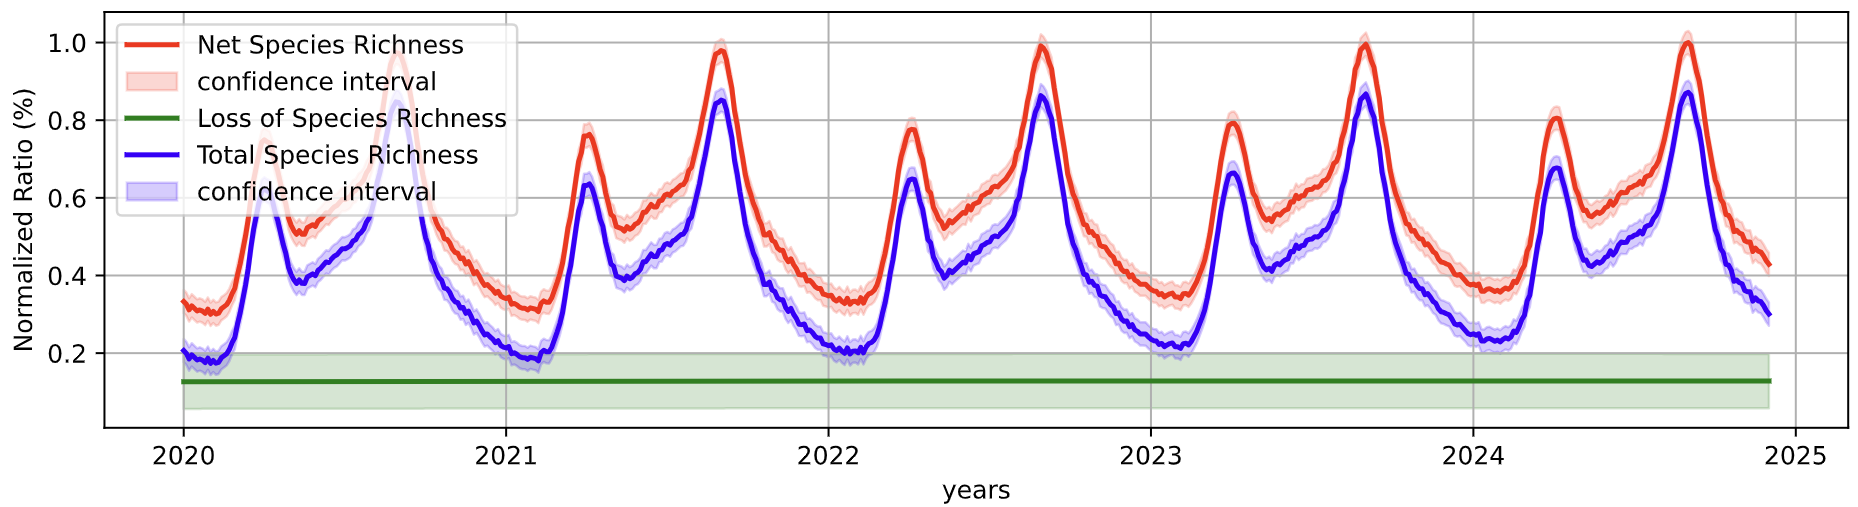
\includegraphics[width=\textwidth]{./figures/shiboqi_hetiban(task3).png}
		\caption{Net \& Total Species Richness when herbicides are removed}
		\label{tk}
	\end{subfigure}
	\begin{subfigure}{\textwidth}
		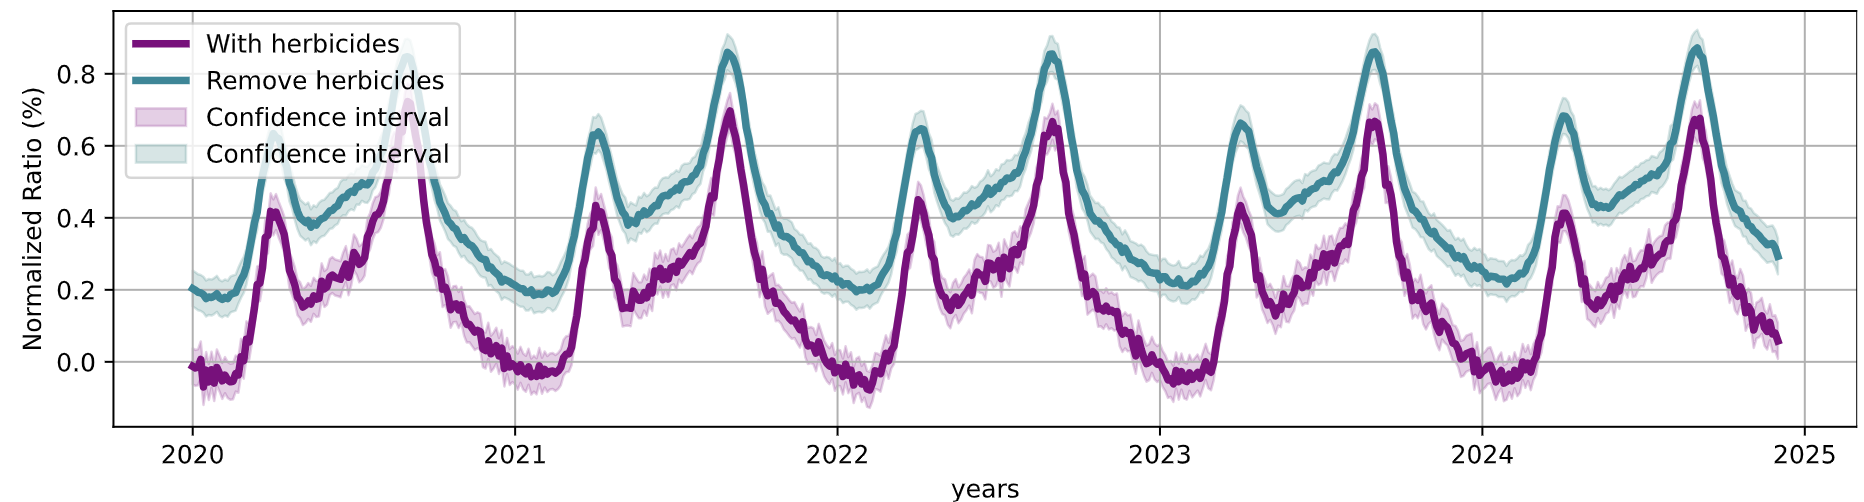
\includegraphics[width=\textwidth]{./figures/shiboqi_Task3(1).png}
		\caption{Comparisons on total species richness before and after herbicides' removal.}
		\label{2}
	\end{subfigure}
	\caption{Effects of herbicide removal on ecosystem stability and species richness.}
	\label{sbq}
\end{figure}


From the perspective of producers, when herbicide usage is discontinued, the growth rate of weeds will evidently increase, leading to a greater diversity of plant species. Additionally, the reduction in harmful chemicals entering the soil promotes the proliferation of soil microorganisms, enhancing soil fertility and subsequently boosting crop yields and the maximum environmental carrying capacity. However, the increase in insect populations may concurrently impose limitations on plant growth, eventually reaching a state of equilibrium. Therefore, we propose the following modifications to the equations in Task 1.
\begin{equation}
	\frac{dB_i}{dt}=\alpha_iB_i(1-\frac{1}{W}\sum_{pro}B_k+\theta_i)-f_{ins-i}B_{insects}-\beta_iB_i
	\label{modified}
\end{equation}
where $\theta_i$ represents the growth-promoting effect of soil microorganisms on species $i$, $\alpha_i=1.285r_i$, $W=1.697K$, $f_{ins-i}=1.276a_{ins-i}$, $\beta_i=0.649d_i$.

However,the aggressive spread of weeds will compete with crops for vital resources like sunlight, water, and soil nutrients, resulting in substantial stress on crop growth.Therefore,We make revisions to the formula \eqref{comp} and define  $q=\frac{\sigma_1}{\sigma_2}$   as the relative competition coefficient between weeds and crops.Based on data analysis, we conclude that $q$ ,in the short term, initially increases over time, then decreases, and finally stabilizes. This indicates that after the cessation of pesticide use, weeds exhibit a stronger competitive ability compared to crops, leading to vigorous growth. Subsequently, due to resource limitations in the environment, their competitive ability diminishes and eventually stabilizes. The initial growth of weeds contributes to the biodiversity of the ecosystem.

From the perspective of consumers,the enhancement of plant diversity and biomass provides animals with a richer source of food resources.The reduction or cessation of pesticide use has led to a significant increase in the abundance of primary consumers, which in turn promotes the growth of secondary consumers. To put it another way, it means $r_{insects}$ and $r_{bird}$ will respectively increase in the formula\eqref{insect} and formula\eqref{bird}. Additionally,the diverse vegetation structures offer more complex habitats for various animal species.These favorable living conditions contribute to the dynamic balance and stable growth of animal populations.The overall improvement of the ecological environment attracts a greater diversity of animal species into the ecosystem, leading to the formation of more intricate food web relationships.This increased complexity significantly enhances the stability and resilience of the ecosystem against disturbances.

We further visualize the impacts of herbicides (and other chemical substances) removal by recalculating total species richness and aforementioned metrics referring to equation \ref{shiboqi_hetiban}. Results are shown in figure \ref{sbq}. From figure \ref{tk} it can be concluded that, loss of species richness triggered by overuse of chemicals are mitigated but still having negative effects on ecosystem stability, while figure \ref{2} demonstrates that herbicide removal could directly contribute to higher biodiversity and stability, where the minimum value has been elevated to 19.8\%.

\subsubsection{Stronger Resistance}
\hspace{2em}According to equation \ref{rts}, we conclude that biodiversity and species richness is positively proportional to ecosystem stability. Additionally, in equation \ref{modified} we optimize formula \ref{original} and infer the removal of herbicides positively facilitates biomass and biodiversity of either producers or consumers, indicating an increase in resistance stability and a decrease in resilience stability, as is illustrated in figure \ref{resistance}

\begin{figure}[h]
	\centering
	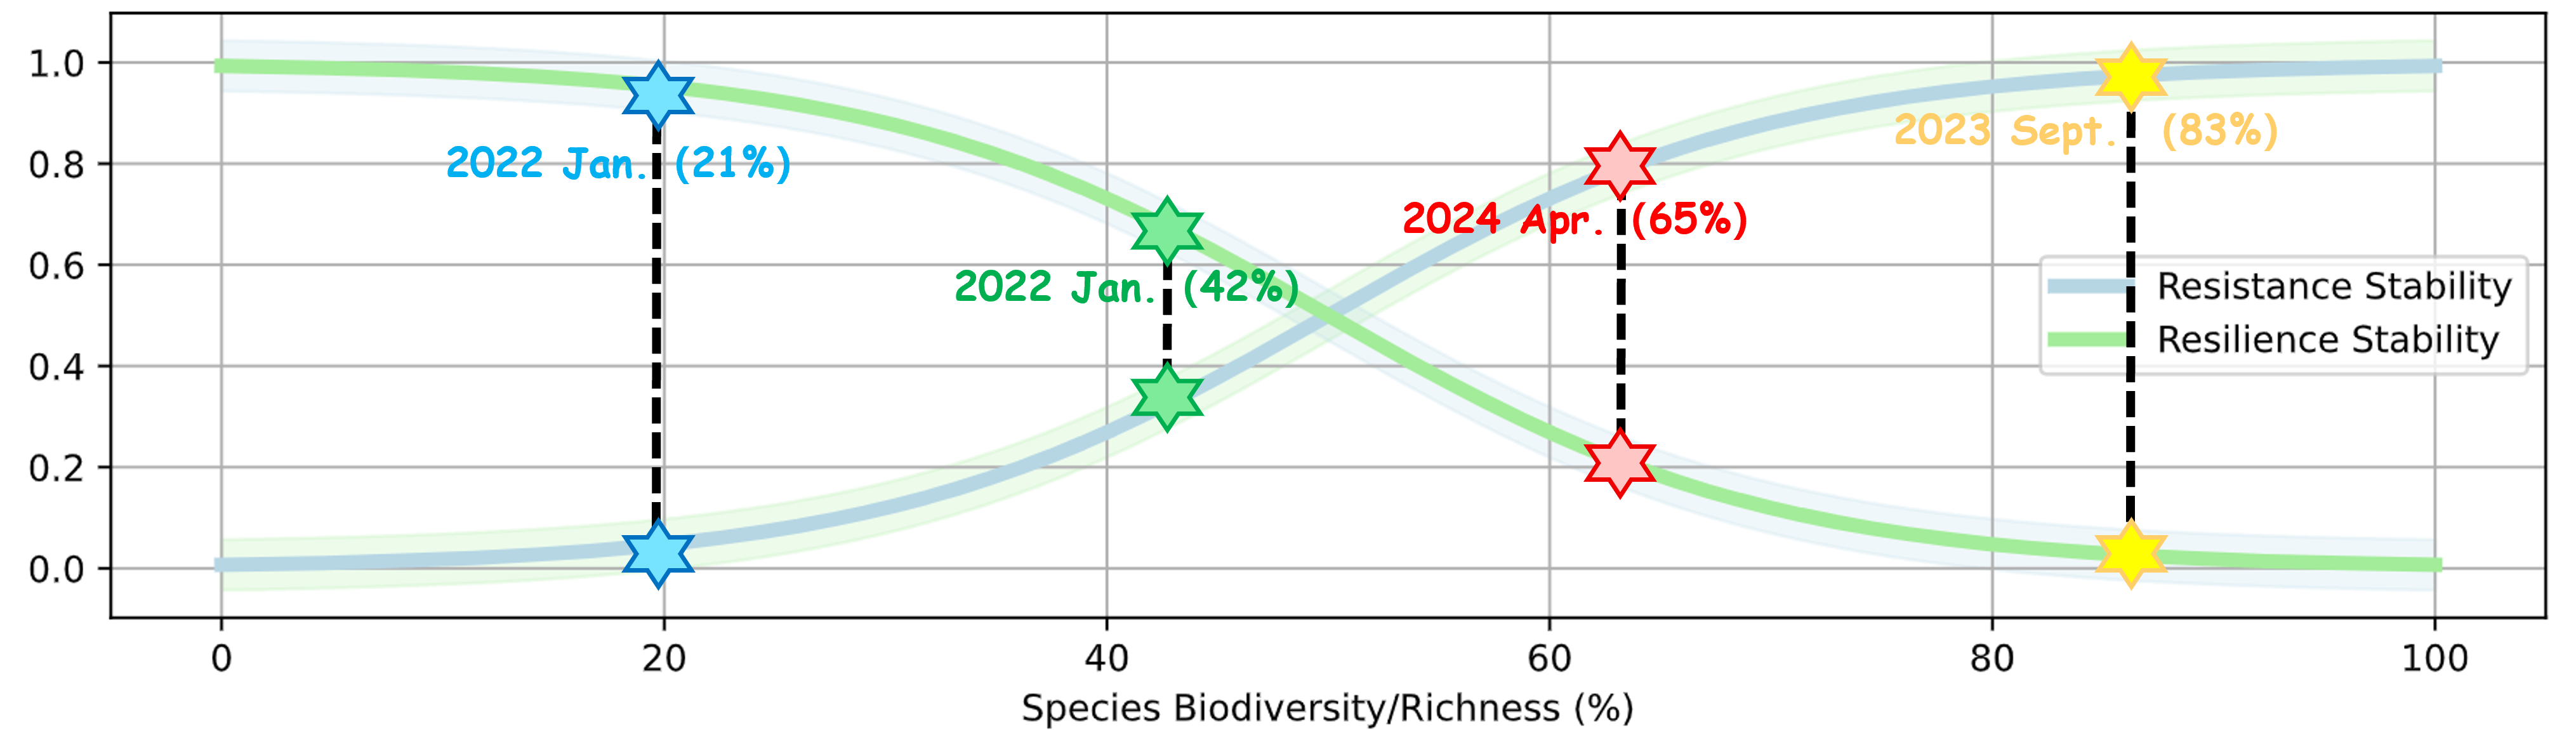
\includegraphics[width=0.8\textwidth]{./figures/resistance(task3).png}
	\caption{$RTS$ and $RLS$ when herbicide are removed.}
	\label{resistance}
\end{figure}

Similar to the stability analysis conducted in section 5.2, let footnote $IH$ stands for ``Including Herbicide'' and $EH$ for ``Excluding Herbicide'', from figure \ref{sbq} and \ref{resistance} obviously we have:$$
\begin{cases}
	RTS_{EH}>RTS_{IH} \\
	RLS_{EH}<RLS_{IH}
\end{cases}\xrightarrow{ }\begin{cases}
	F_{EH}>F_{IH} \\
	(t_1-t_0)_{EH}<(t_1-t_0)_{IH}
\end{cases}\xrightarrow{ }TES_{EH}<TES_{IH}
\xrightarrow{ }Stability_{EH}>Stability_{IH}
$$

Therefore, considering the short term analysis where \textbf{the competitive impacts of weeds against crops are dismissed}, we reach to the conclusion that: 

\begin{center}
	\textit{
	When herbicide is removed, the ecosystem will become more stable. The deeper mechanism can be explained from two perspectives. On the one hand, removal of herbicide and other chemicals reduce the loss of species richness by nourishing consumers and predators in food web (section 6.1.1), which in turn contributes to a higher biodiversity and system stability; On the other hand, removal of herbicide increases resistance stability and decreases resilience stability (section 6.2.2), which leads to an elevation in overall ecosystem stability. \textbf{However, the balance is doomed to break considering the drastic increase in weeds, powerful competitors against crops for nutrients.}
	}
\end{center}
	\subsection{\textit{``Bring the bats back! ''}---A Long Term Solution}
\hspace{2em}In this section, we solve the ``weeds problems'' which destroy the ecological balance by introducing bats as the biological controlling methodology. Through integrating the Broadened Pascal's Triangle and convolution kernels, we manage to quantify and visualize the beneficial effects bats bring to agricultural system and the interactions between bats, plants and predators. A similar species is found by rebuilding the kernels, whose impacts to the surrounding environments can be revealed in its kernel size and value.

\subsubsection{Bats' Interactions with Ecosystem}
\hspace{2em}\textbf{Review of core concepts.} Convolution kernel reveals the dynamic interactions between certain subjects and its surrounding environments, particularly when the effects of selected subject are required to be evaluated. 
For instance, let $K$ be the kernel with a receptive field of $3\times 3$, $I$ be the $10\times 10$ input convolution area, then we have equation \ref{juanji}, where $i,j$ represent line and column index of output signal, and $m,n$ stand for counterparts of the convolution kernel.  
\begin{equation}
	K=\begin{bmatrix}
	K_{11} & K_{12} & K_{13} \\
	K_{21} & K_{22} & K_{23} \\
	K_{31} & K_{32} & K_{33} 
\end{bmatrix},\ I=\begin{bmatrix}
	I_{11} & I_{12} & \dots & I_{19} \\
	I_{21} & I_{22} & \dots & I_{29} \\
	\vdots & \vdots & 		& \vdots \\
	I_{91} & I_{92} & \dots & I_{99} \\
\end{bmatrix},\ O=\sum_{m=1}^{3}\sum_{n=1}^{3}K_{mn}\cdot I_{i+m-1,j+n-1}
\label{juanji}
\end{equation}


Broadened Pascal's Triangle is proposed in section 5.1, where each value in triangles stands for the normalized ratio of total species richness.

\textbf{Model Establishment. }Considering that bats play a complicated role in food webs, we design three ``Bat Kernels'' respectively for insect layer, plant layer and predator layer. The three layers represent biomass of respective creatures, calculated in the following fashion, where the coefficients are extracted from figure \ref{chemics}.
\begin{equation}
	\begin{cases}
Plant\ Layer = 0.864\times Total\ richness, \\ Insect\ Layer = 0.071\times Total\ Richness, \\ Predator\ Layer = 0.065\times  Total\ Richness.
	\end{cases}\label{ca}
\end{equation}


Since bats are modeled as insectivores that control pest populations and flourish plants, convolution kernels are designed as figure \ref{kernel}. Each value in kernel is proposed through rigorous evaluation of bats' impacts to surrounding environments. Let $\omega_{ij}(i,j\in{1,2,3})$ stands for the numbers in kernels, we define $\omega_{ij}>1$ as ``bats support the objects' reproduction'' while $\omega_{ij}<1$ the opposite. Additionally, $\omega_{ij}\propto supporting\ extent$. Obviously, bats stimulate plant reproduction by clearing pests and certain competitor species, so $\omega_{ij}$ in plant layer kernel all surpass 1. In section 4.1, our EEIM model describes bats as predators to insects while competitors against other herbivores. Therefore, the majority of $\omega_{ij}$ in insect layer kernel and predator counterparts are less than 1, since the existence of bats worsens their living conditions.
\begin{figure}[h]
	\centering
	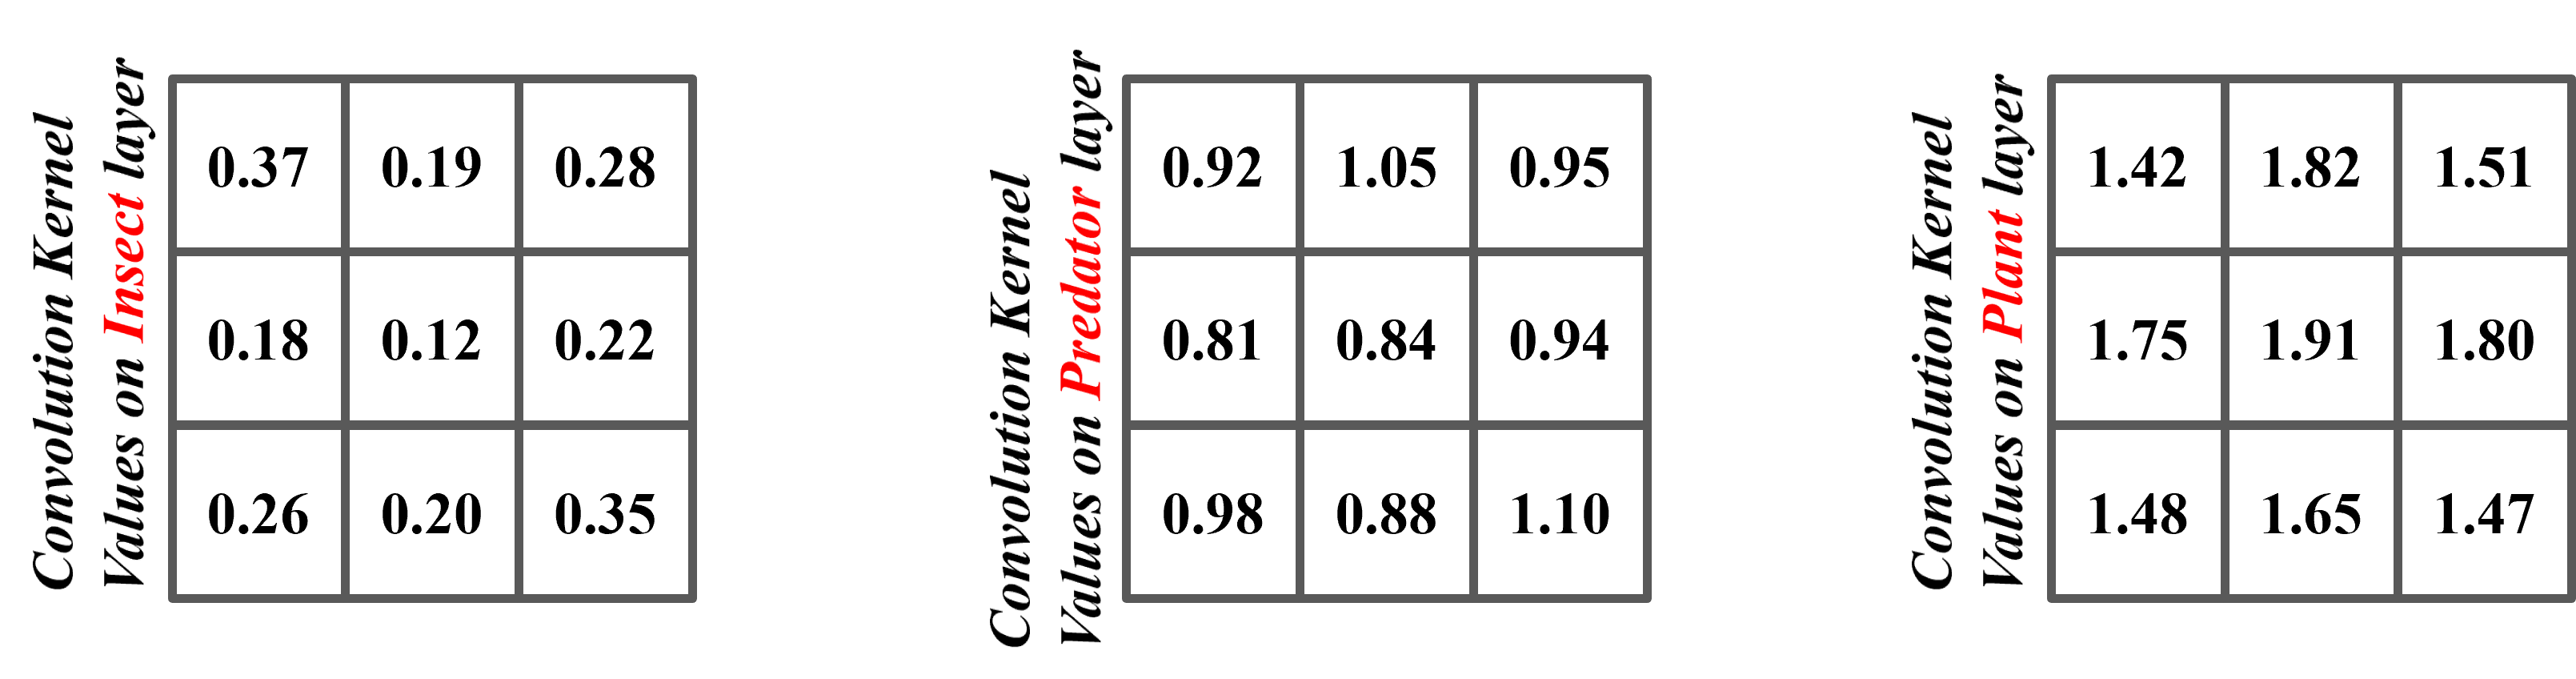
\includegraphics[width=0.9\textwidth]{./figures/kernel(task3).png}
	\caption{Three $3\times3$ convolution kernels for different layers, namely \textbf{Bats Kernels.}}
	\label{kernel}
\end{figure}

Then the layers before introducing bat kernels are calculated based on equation \ref{ca}, as is demonstrated in figure \ref{layers}. Finally we convolve the kernels on corresponding layers (equation \ref{juanji}, figure \ref{haokun}).

\begin{figure}[h]
	\centering
	\begin{subfigure}{0.22\textwidth}
		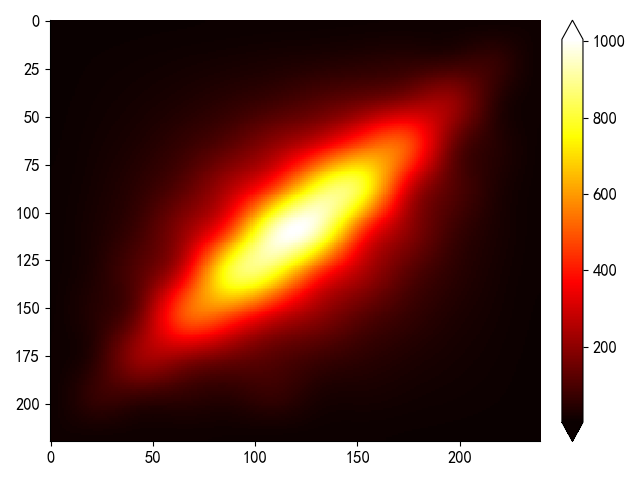
\includegraphics[width=\textwidth]{./figures/primitive(task3).png}
		\caption{Total Richness}
	\end{subfigure}
	\begin{subfigure}{0.22\textwidth}
		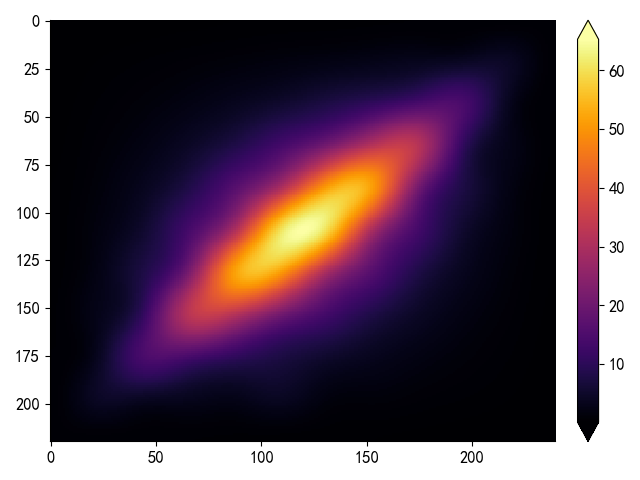
\includegraphics[width=\textwidth]{./figures/predator(task3).png}
		\caption{Predator Layer}
	\end{subfigure}
	\begin{subfigure}{0.22\textwidth}
		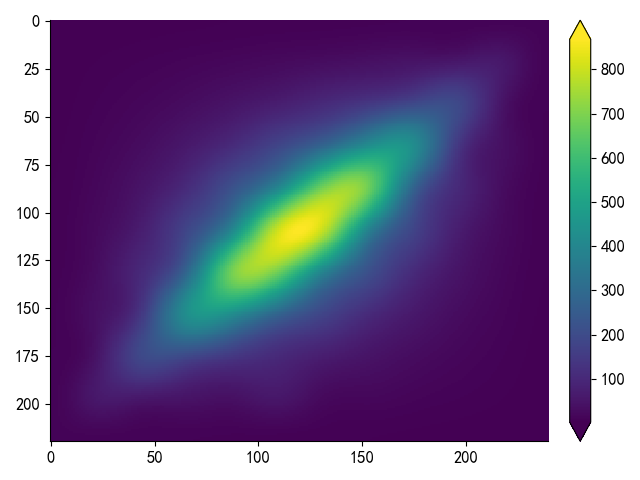
\includegraphics[width=\textwidth]{./figures/plant(task3).png}
		\caption{Plant Layer}
	\end{subfigure}
	\begin{subfigure}{0.22\textwidth}
		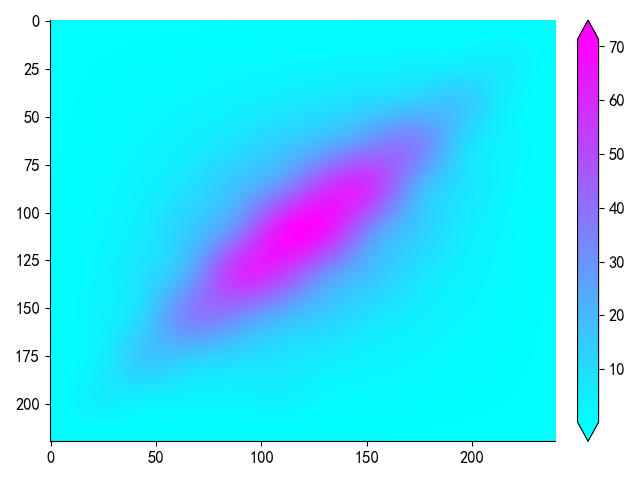
\includegraphics[width=\textwidth]{./figures/insect(task3).png}
		\caption{Insect Layer.}
	\end{subfigure}
	\caption{Calculation of Layers before bat kernel convolution.}
	\label{layers}
\end{figure}

\begin{figure}[h]
	\centering
	\begin{adjustwidth}{-0.115\textwidth}{}
			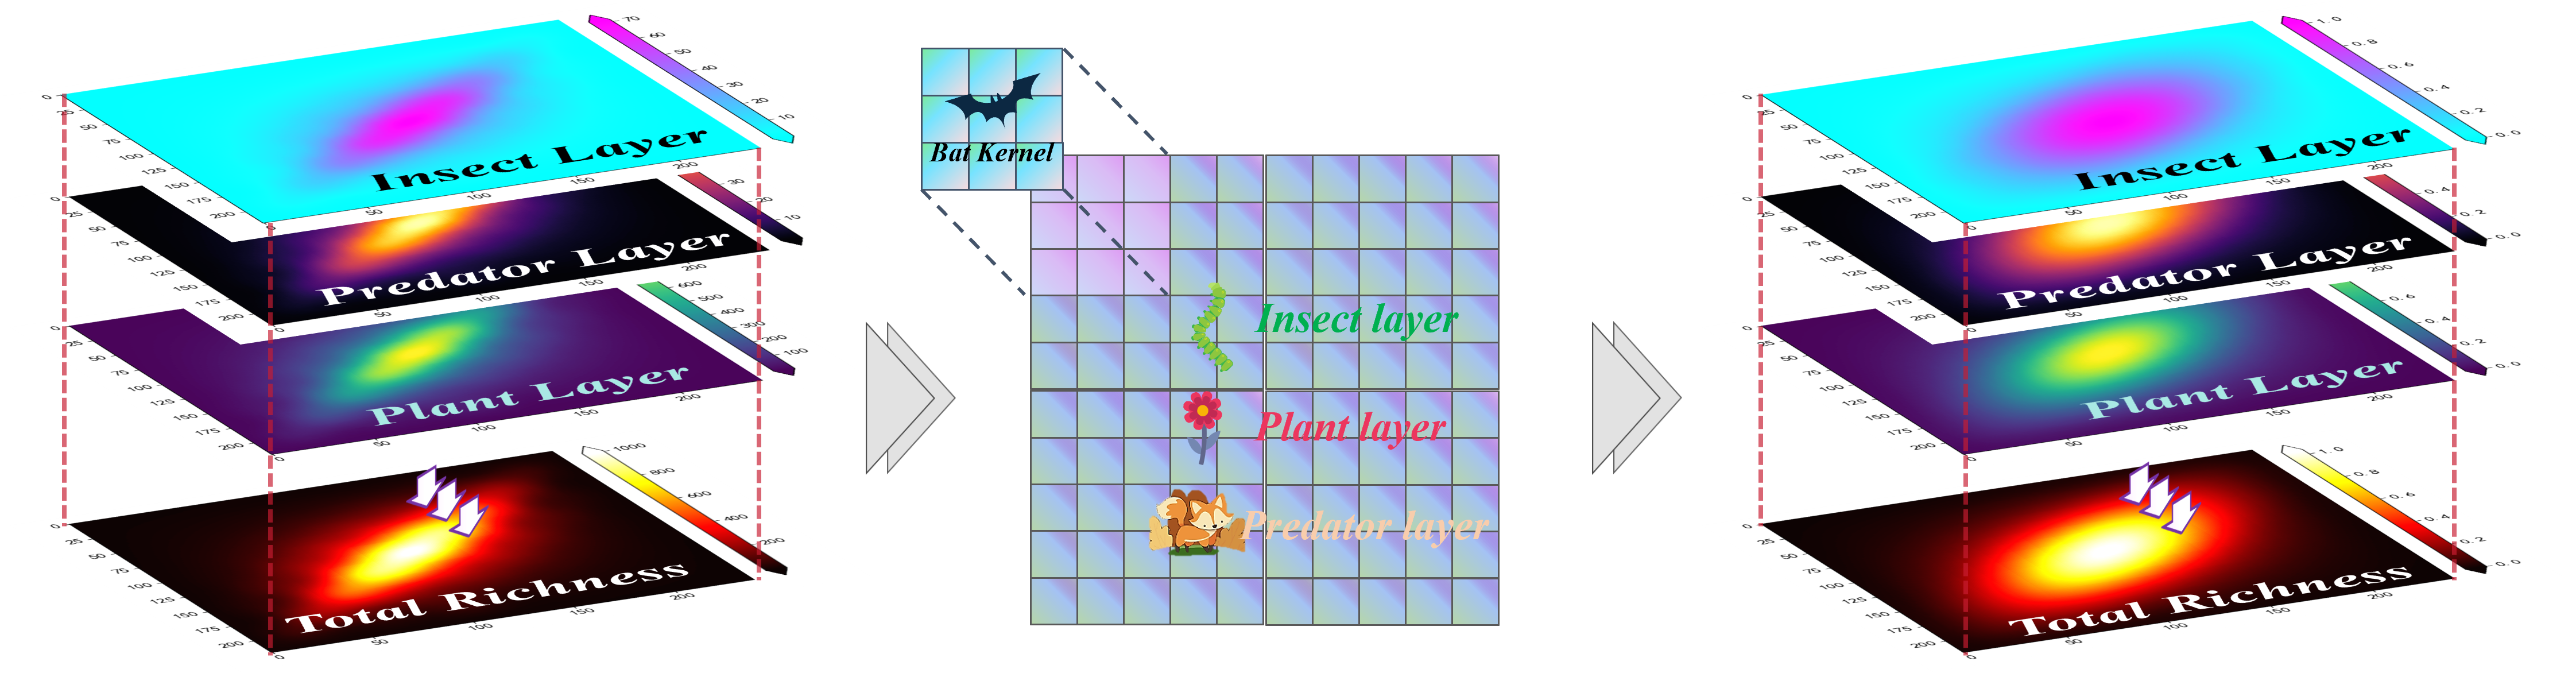
\includegraphics[width=1.2\textwidth]{./figures/convolve(task3).png}
	\end{adjustwidth}
	\caption{Bat kernel convolution on different layers and the integration of corresponding layers.}
	\label{haokun}
\end{figure}
\textbf{Explanations on Bats' Interaction with other creatures. }Take pests as the example. From figure \ref{haokun} it can be observed that pests and insects become more evenly distributed after the introduction of bats, which can be simulated by figure \ref{moni}.
\begin{figure}[h]
	\centering
	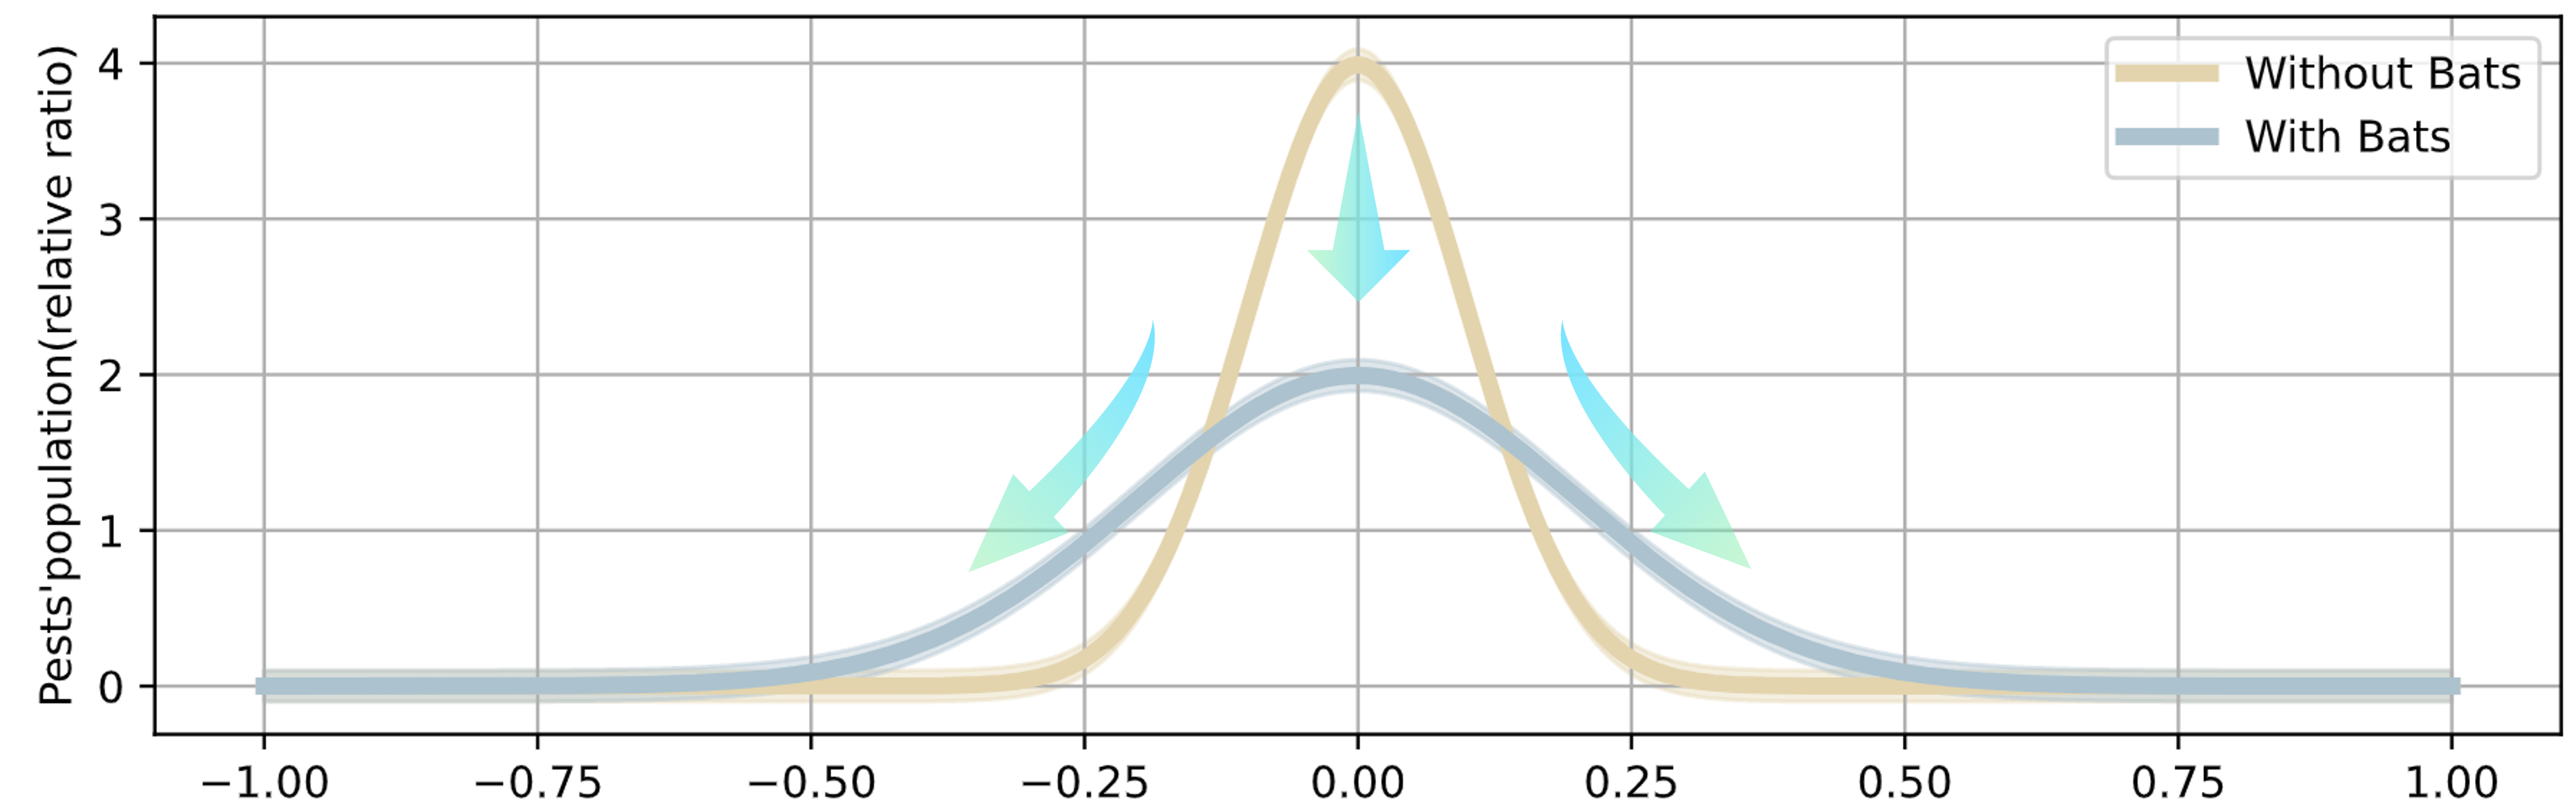
\includegraphics[width=0.85\textwidth]{./figures/Insects_expl(task 3).png}
	\caption{With and without bats considering geographical distribution of pests.}
	\label{moni}
\end{figure}

From figure \ref{moni}, before bats appear, pests and insects mainly survive in the central regions where crops flourish and nutrients are more than sufficient. The introduction of bats, however, turns the tables. Not only does the maximum population of pests deteriorated but they are also compelled to move into marginalized areas to escape the bats, leading to a evenly separated distribution that roughly satisfies $\mathcal{N}(0,0.2)$. Such phenomenon is also observed in figure \ref{haokun}, where the brightest areas of heat-map enlarges. 

Similar analysis can as well be conducted on predators and plants, culminating in similar conclusions which align with the results illustrated in figure \ref{haokun}.

\subsubsection{the Ecosystem Stability Outcome}
\hspace{2em}Although a prosperous biodiversity and species richness is gladly expected in a mature agricultural ecosystem and we have analyzed that bats definitely contributes to such wishes, it does not, however, necessarily lead to the stability.

In section 5.2 we introduce the Ecosystem Stability Model which comprises three sub-variables: Resistance Stability ($RTS$), Resilience Stablity ($RLS$) and Total Ecosystem Stablity ($TES$). Considering the primary goal of agricultural ecosystems is to harvest, neither $RTS>>RLS$ or $RTS<<RLS$ is what we expect. For instance, when $RTS\to0$, the ecosystem is too weak to stand any disturbance (e.g., harsh winters); when $RLS\to0$, the ecosystem suffers severe economic losses when extreme weather events attack since the system is too complicated to recover. In figure \ref{x} and \ref{resistance}, we correlate $RLS$ and $RTS$ with species richness, which means that, in order to maintain a stable agricultural ecosystem, biodiversity and species richness have to be confined within a finite range. Only when richness falls into this interval can an ecosystem sustain stability.

\begin{figure}[h]
	\centering
	\begin{subfigure}[b]{0.4\textwidth}
		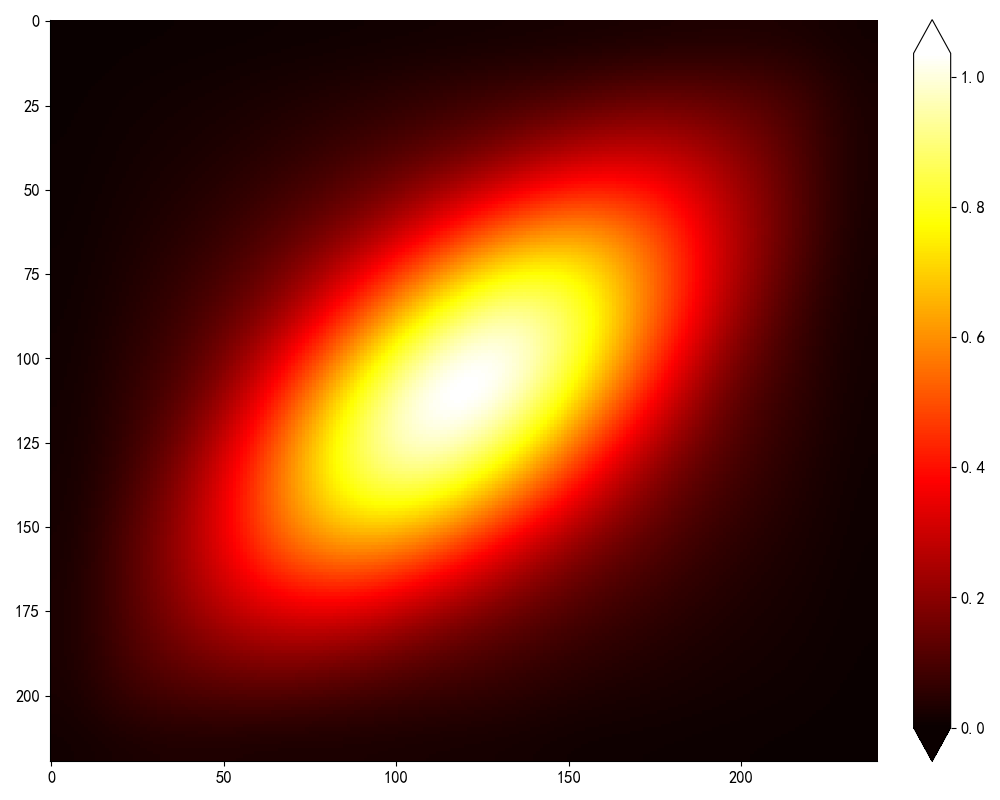
\includegraphics[width=\textwidth]{./figures/withbats(task3).png}
		\caption{Species Richness distribution.}
	\end{subfigure}
	\begin{subfigure}[b]{0.477\textwidth}
		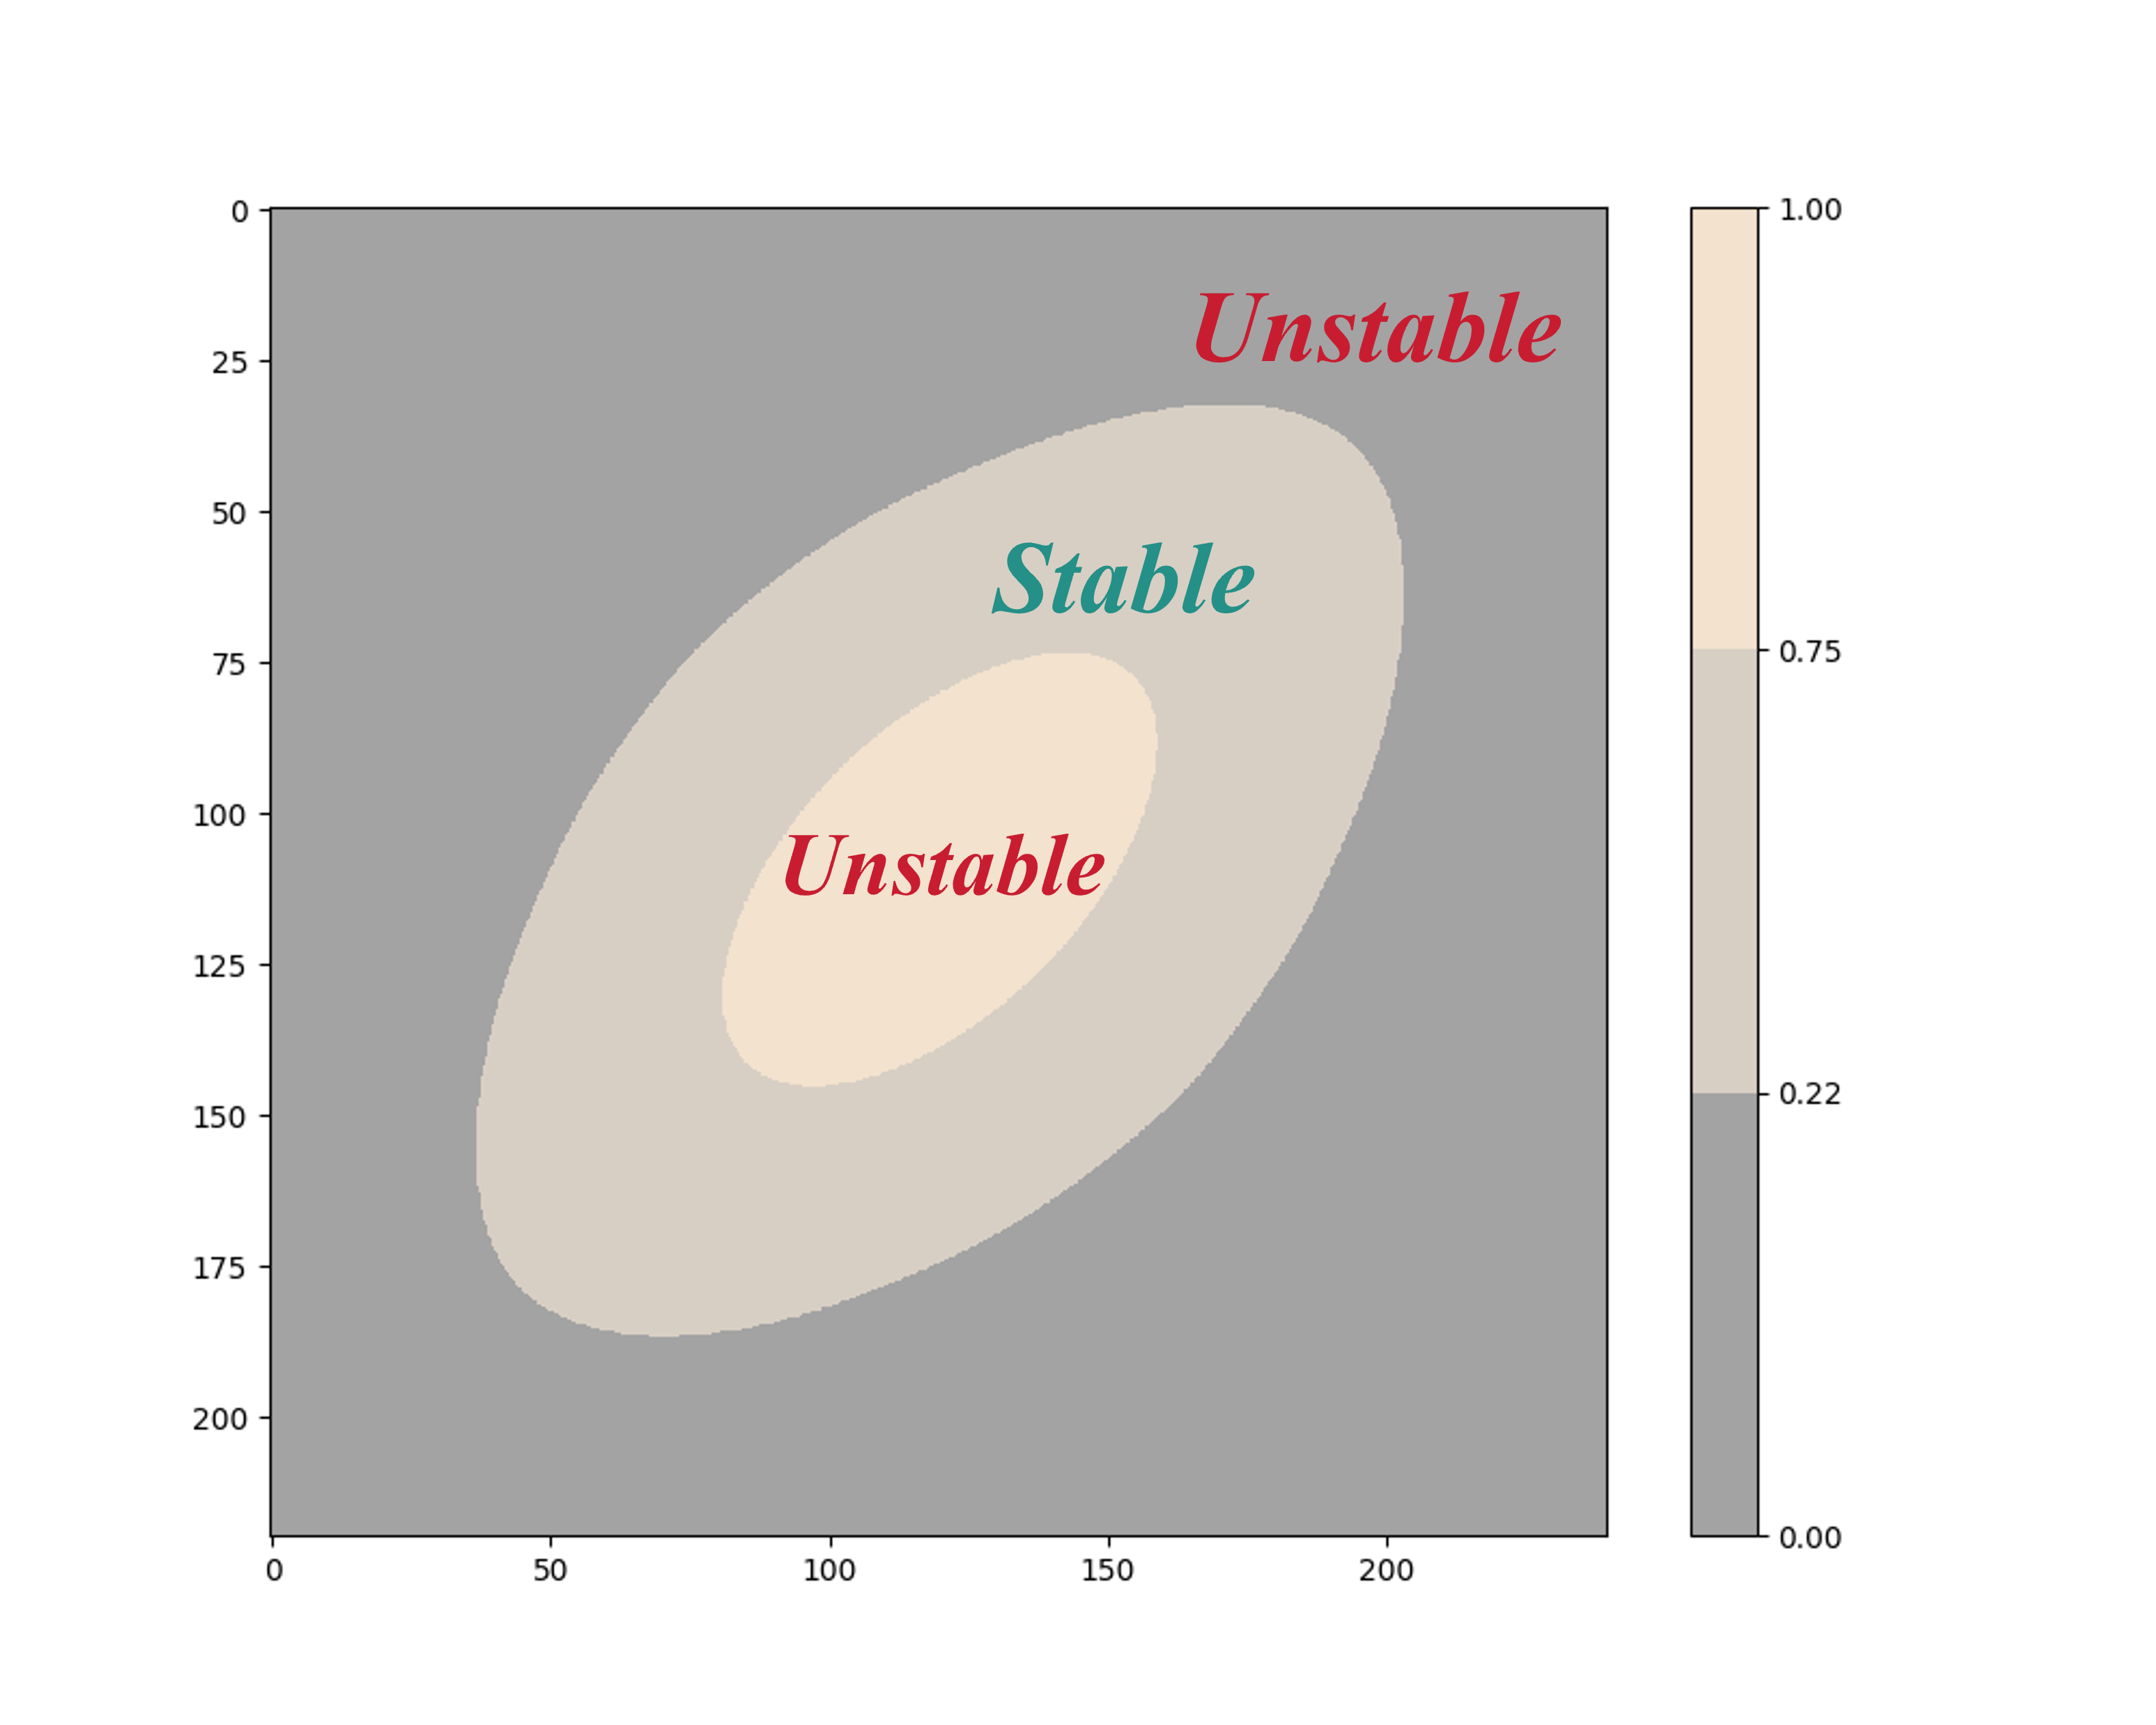
\includegraphics[width=\textwidth,trim=0cm 1.4cm 0cm 0cm, clip]{./figures/stability_interval(task3).png}
		\caption{Categories of stability}
	\end{subfigure}
	\caption{Ecosystem stability interval: $Species\ Richness\in[22\%,75\%]$ }
	\label{jiayou}
\end{figure}

Referring to figure \ref{x} and \ref{resistance}, we acquire equation \ref{cheng}, where $Species\ Richness$ corresponds to the $y$-coordinates of figure \ref{sbq}, namely our food web model output.

\begin{equation}
	\begin{cases}
		Species\ Richness\in[22\%,75\%]\xrightarrow{}\text{\textbf{Stable}} \\
		Species\ Richness\in[0\%,22\%)\cup(75\%,100\%]\xrightarrow{}\text{\textbf{Unstable}}
	\end{cases}
	\label{cheng}
\end{equation}

In summary, the introducing of bats solves the ``weeds problem'' which might trigger ecosystem instability after herbicide removal. However, even though bats' positive interactions with plants, predators and insects do contribute to an increased biodiversity and species richness to a certain extent which seems to stabilize the ecosystem, datas demonstrate that only when richness falls within a finite range ($[22\%,75\%]$) can an ecosystem authentically evolves into a stable one.
\subsection{Grass Snake---\textit{``Bats are not alone.''}}
\hspace{2em}Grass Snake is a species commonly found in agricultural fields and surrounding environments, feeding on frogs, small reptiles, etc. It is a carnivorous snake with negligible predation on insects, forming a striking contrast with bats whose major food resource is insects.


As a higher-level predator in food webs, grass snake brings ecosystems back into balance by preying on harmful animals (e.g., mice). However, it only indirectly controls pest population, which differs from bats. Therefore, we redesign the Snake Kernels referring to principles listed in figure \ref{kernel}. The Convolution kernels are illustrated in figure \ref{snake}.
\begin{figure}[h]
	\centering
	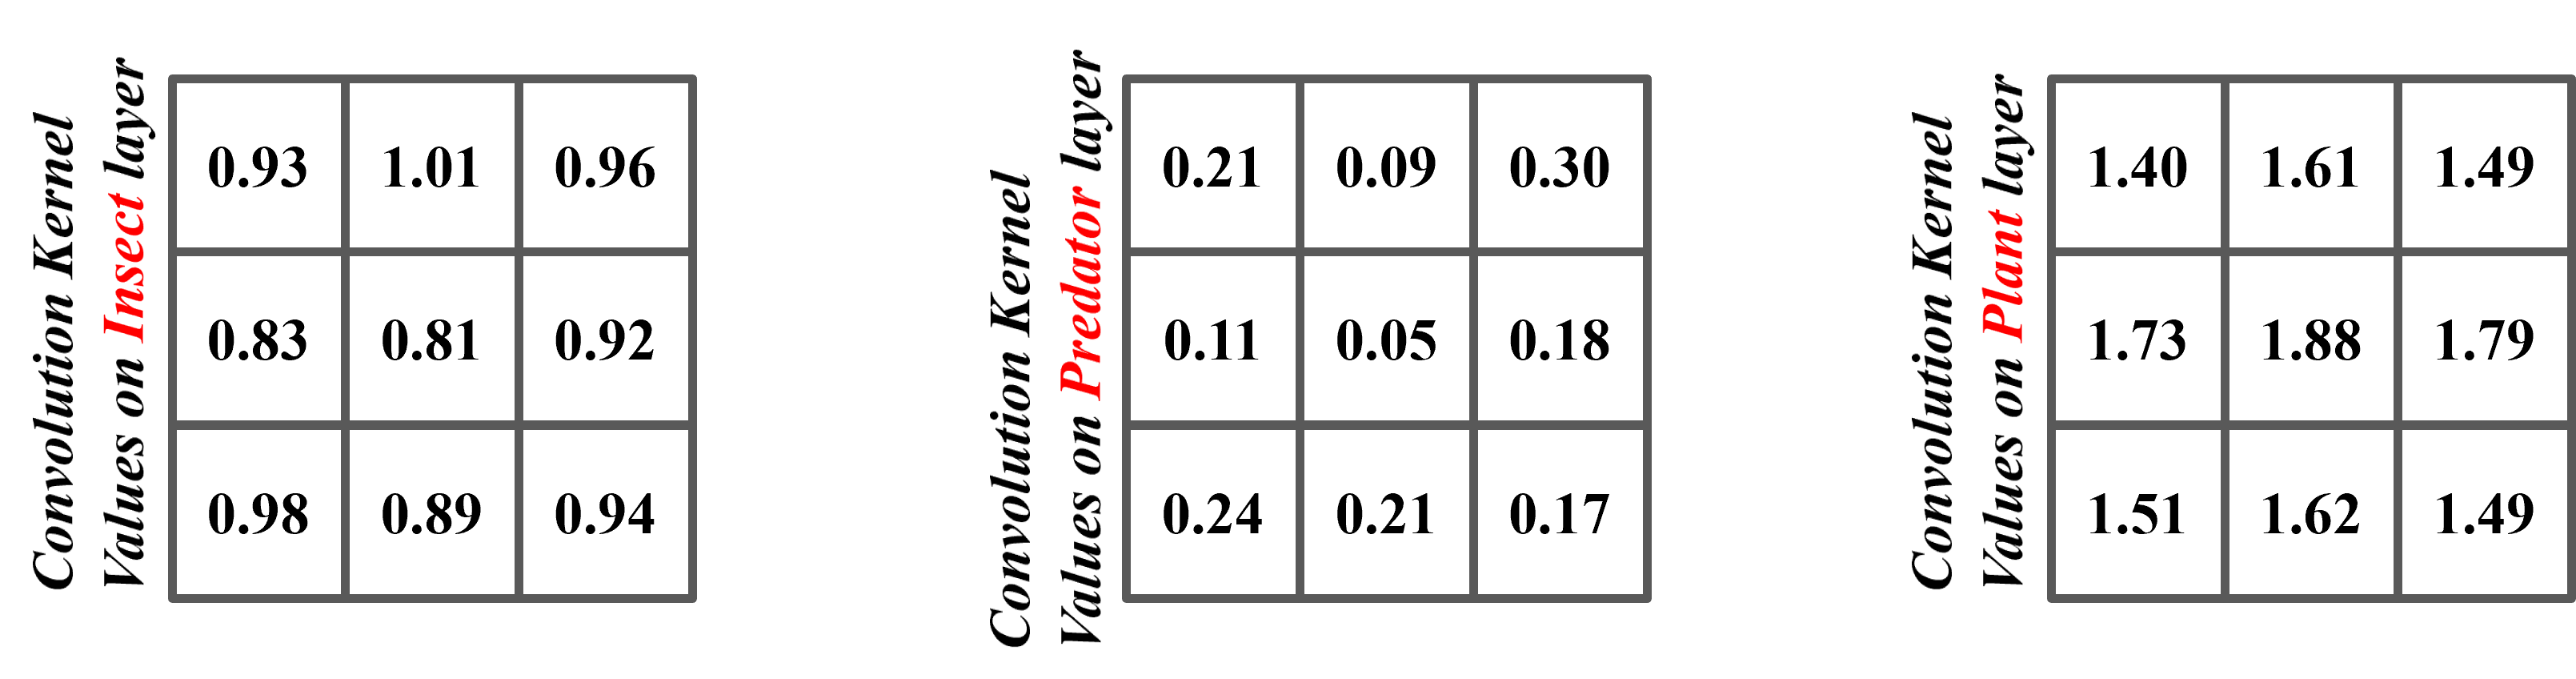
\includegraphics[width=\textwidth]{./figures/snake_kernel(task3).png}
	\caption{Snake Kernel.}
	\label{snake}
\end{figure}

After the convolution calculations similar to figure \ref{haokun}, we further compare the differences between bat kernel results and the snake kernel counterparts, which could reveal their discrepancy in essence, as is demonstrated in figure \ref{ch}. We quantificationally determine species richness by measuring the geological distance in graphs, acquiring: $c_1=c_2,\ d_1>d_2,\ b_1\approx b_2,\ a_1<a_2$. The results feature strong practical meaning.
\begin{figure}[h]
	\centering
	\begin{subfigure}{0.47\textwidth}
		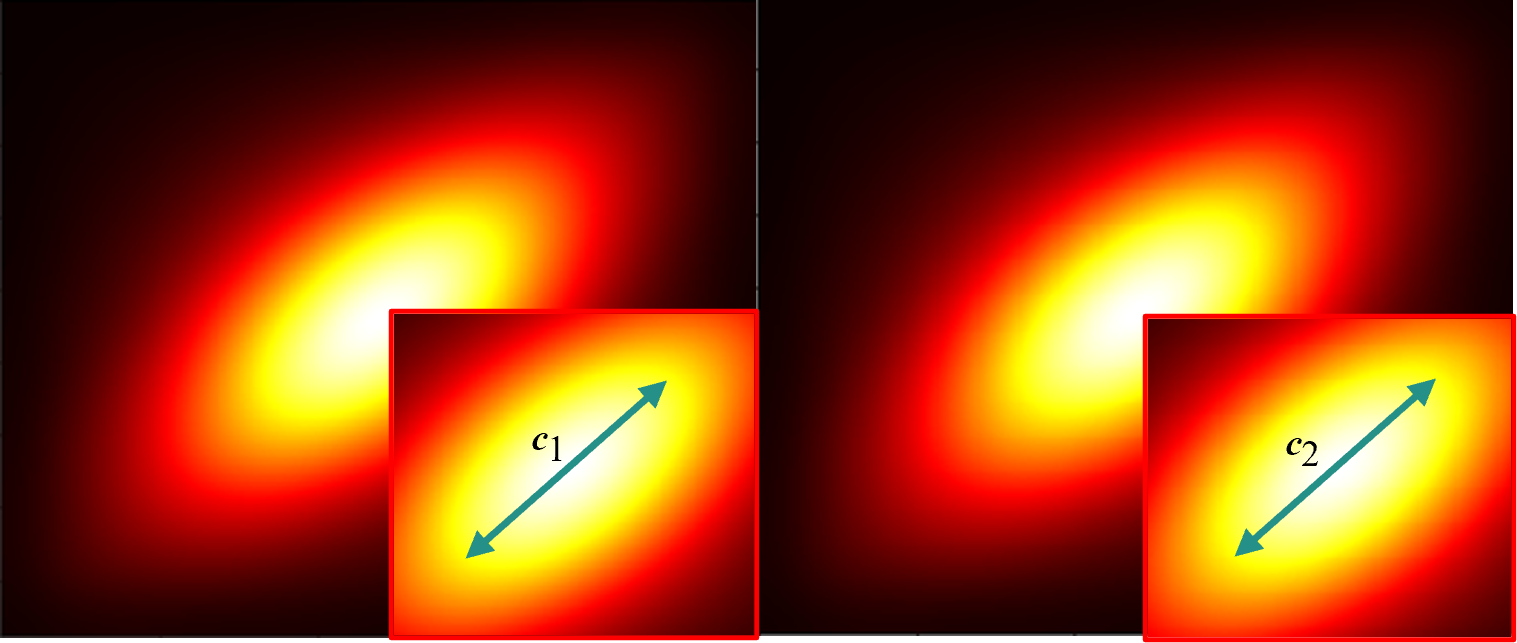
\includegraphics[width=\textwidth]{./figures/total(task3).png}
		\caption{Total Species Richness.}
	\end{subfigure}
	\begin{subfigure}{0.47\textwidth}
		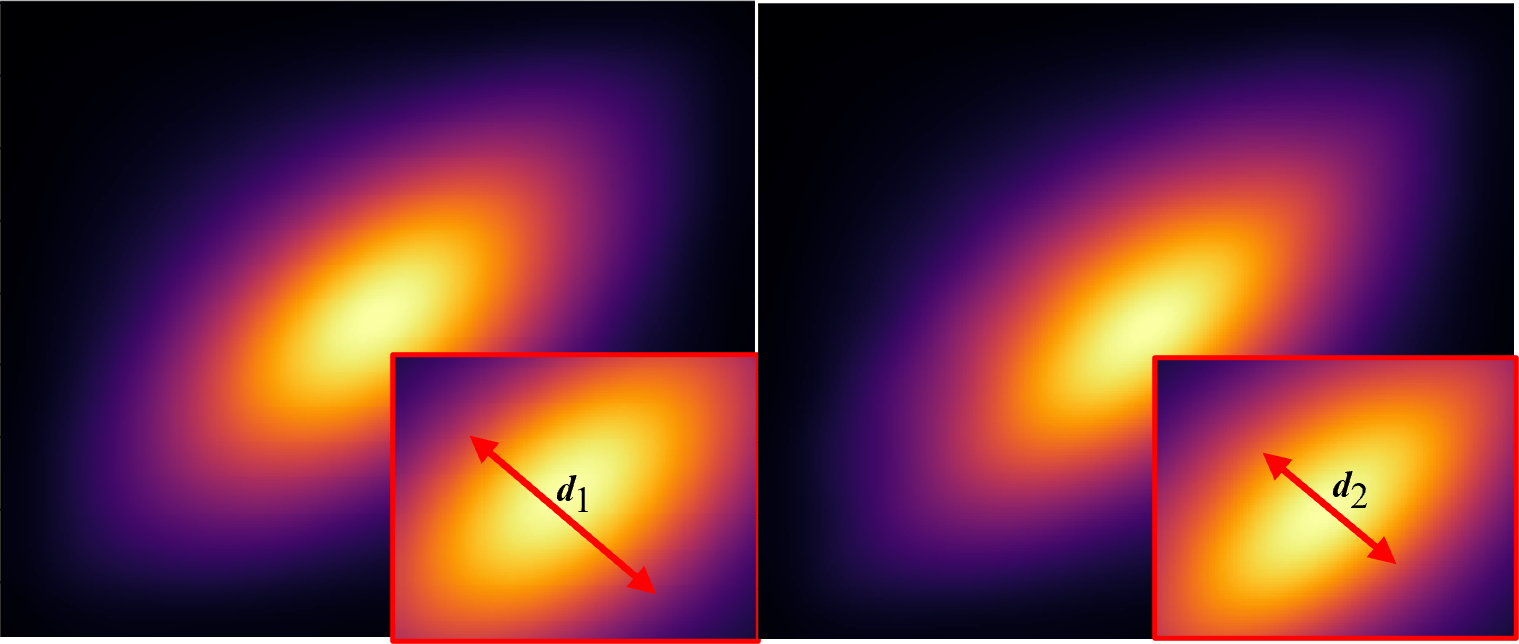
\includegraphics[width=\textwidth]{./figures/pred(task3).png}
		\caption{Predator Layer.}
		\label{pred}
	\end{subfigure}
	\begin{subfigure}{0.47\textwidth}
		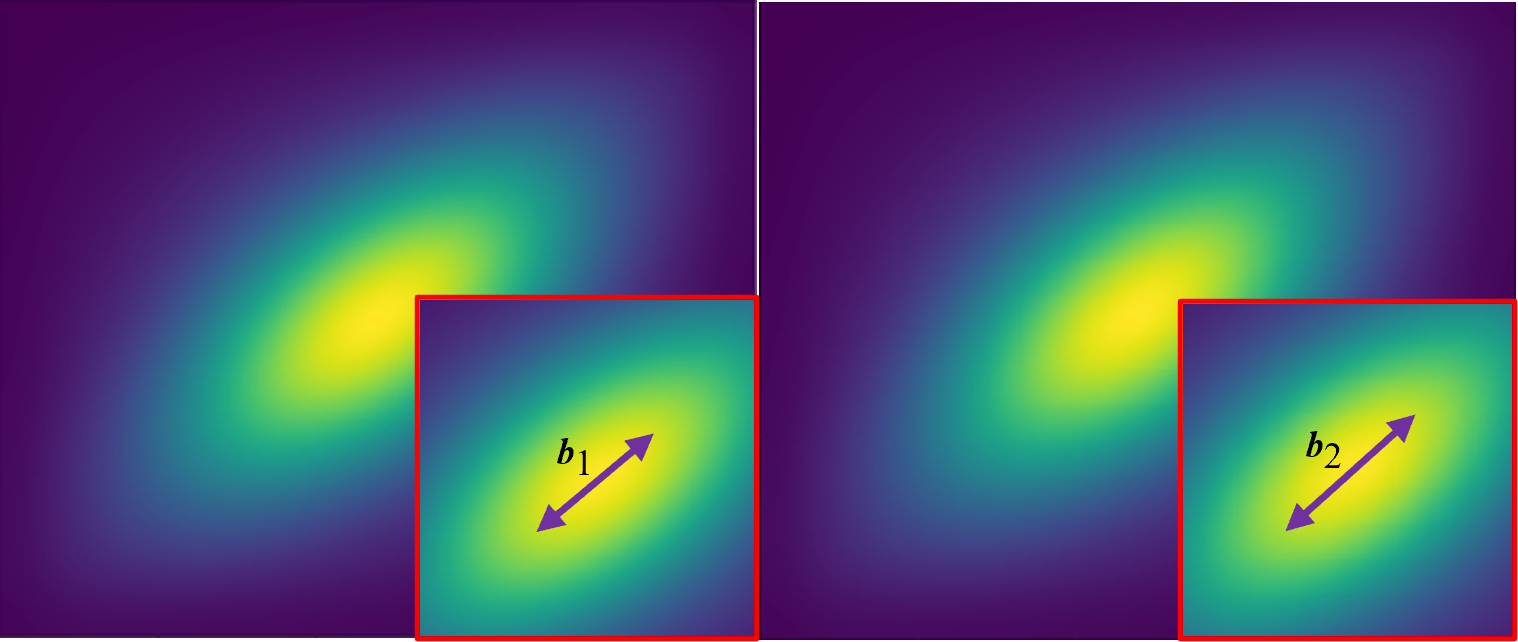
\includegraphics[width=\textwidth]{./figures/plt(task3).png}
		\caption{Plant Layer.}
		\label{zhiwu}
	\end{subfigure}
	\begin{subfigure}{0.47\textwidth}
		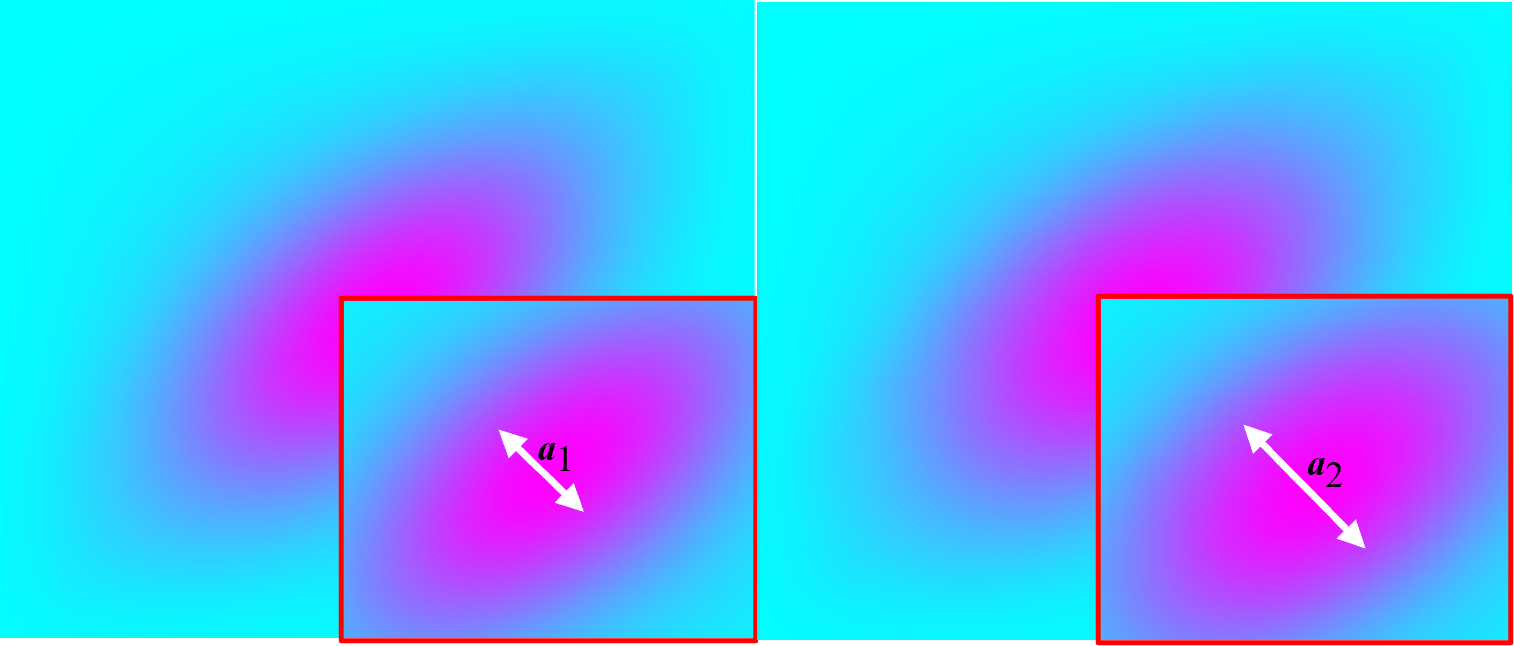
\includegraphics[width=\textwidth]{./figures/insec(task3).png}
		\caption{Insect Layer.}
		\label{chong}
	\end{subfigure}
	\caption{Comparisons between bats and snakes, where the left figures stand for snake kernels' convolution results and right ones represent bats (extracted from figure \ref{haokun}).}
	\label{ch}
\end{figure}

Firstly, from figure \ref{moni} and \ref{haokun} we reach to the conclusion that, if the animal being introduced facilitate ecosystem stability and drive the noxious creatures to marginal habitats, species richness distribution will become more even than before. In heat-maps such as figure \ref{jiayou}, the brightness region appears broader on the graph. In figure \ref{ch} from  $c_1=c_2$, we conclude that grass snakes and bats have similar impacts on ecosystem stability considering total species richness and biodiversity, while on the detailed food web components, two species differ. As a higher-level predator, grass snakes pose deeper impacts on other predators while bats don't, causing $d_1>d_2$ in figure \ref{pred}; Since both species all benefit agricultural system, the differences of their effects on plants and crops is negligible, resulting in $b_1\approx b_2$ in figure \ref{zhiwu}; As for the pests and other insects, bats influence more than grass snakes since bats are lower-level predators and could directly impact insect population through preying while grass snakes cannot, culminating in $a_2>a_1$ in figure \ref{chong}. 

In summary, grass snakes could facilitate the agricultural ecosystem stability just as bats do. However, their inner mechanisms contrast significantly. Bats, as lower-level predators, directly control pest population through preying  and have negligible impacts on trophic level consumers; Grass snakes, as higher-level predators, directly impact other consumers and indirectly control the pest population generally relying on the chain-reactions of food webs. Both species have similar effects on plants and crops, since the primary goal of an agricultural system is to harvest.

	%%%%%%%%%% 正文结束 %%%%%%%%%%%%
	%%%%%%%%% 参考文献开始 %%%%%%%%%%%%
	\newpage
	\begin{thebibliography}{00}
		
		\bibitem{1} % 第一个参考文献，以此类推
		
		
		\bibitem{2} % 第二个参考文献
		
		
		\bibitem{3} % 第二个参考文献
		
	\end{thebibliography}
	%%%%%%%%% 参考文献结束 %%%%%%%%%
	%%%%%%%%% 全文结束 %%%%%%%%%%%%%
\end{document}
\end
